\section{eo\-Pop\-Eval\-Func$<$ EOT $>$ Class Template Reference}
\label{classeo_pop_eval_func}\index{eoPopEvalFunc@{eoPopEvalFunc}}
eo\-Pop\-Eval\-Func: This abstract class is for GLOBAL evaluators of a population after variation.  


{\tt \#include $<$eo\-Pop\-Eval\-Func.h$>$}

Inheritance diagram for eo\-Pop\-Eval\-Func$<$ EOT $>$::\begin{figure}[H]
\begin{center}
\leavevmode
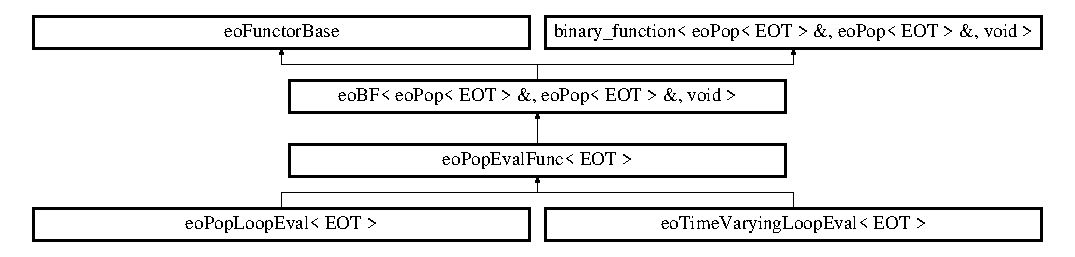
\includegraphics[height=3.01075cm]{classeo_pop_eval_func}
\end{center}
\end{figure}


\subsection{Detailed Description}
\subsubsection*{template$<$class EOT$>$ class eo\-Pop\-Eval\-Func$<$ EOT $>$}

eo\-Pop\-Eval\-Func: This abstract class is for GLOBAL evaluators of a population after variation. 

It takes 2 populations (typically the parents and the offspring) and is suppposed to evaluate them alltogether

Basic use: apply an embedded {\bf eo\-Eval\-Func}{\rm (p.\,\pageref{classeo_eval_func})} to the offspring

Time-varying fitness: apply the embedded {\bf eo\-Eval\-Func}{\rm (p.\,\pageref{classeo_eval_func})} to both offspring and parents

Advanced uses: Co-evolution or \char`\"{}parisian\char`\"{} approach, or ...

Basic parallelization (synchronous standard evolution engine): call the slaves and wait for the results 



Definition at line 49 of file eo\-Pop\-Eval\-Func.h.

The documentation for this class was generated from the following file:\begin{CompactItemize}
\item 
eo\-Pop\-Eval\-Func.h\end{CompactItemize}
